\section*{HS/13. feladat: Hőátszármaztatás síkfalon keresztül}
\addcontentsline{toc}{section}{HS/13. feladat: Hőátszármaztatás síkfalon keresztül}

\begin{tabular}{ | p{2cm} | p{14cm} | } 
	\hline
	Név & Vasáros Mátyás \\ 
	\hline
	Szak & Mechatronikai mérnöki alapszak\\ 
	\hline
	Félév & 2019/2020 II. (tavaszi) félév \\ 
	\hline
\end{tabular}
\vspace{0.5cm}

\noindent A feladat egy nagy kiterjedésű homogén síkfal állandósult állapotú hőátszármaztatása esetén kiszámítani a hőáramsűrűséget és a fal két oldalán a hőfokesést. A fal két oldalán ismert a hőmérséklet ezek $T_{1}=\SI{400}{\degreeCelsius}$ és $T_{4}=\SI{200}{\degreeCelsius}$. A fal egyik oldalán a hőátadási tényező értéke az átváltás után $\alpha_1$ a másik oldalon $\alpha_2$, a fal hőátadási tényezője $\lambda$. A fal vastagsága $\delta=\SI {16}{\milli\meter}=\SI {0,016}{\meter}$.

\begin{equation*}
	\alpha_1=\SI{1162}{\watt\per\meter\squared\kelvin},
\quad 
	\alpha_2=\SI{581,5}{\watt\per\meter\squared\kelvin},
\quad 
	\lambda=\SI{44,652}{\watt\per\meter\kelvin}
\end{equation*}

\noindent\hrulefill

\begin{figure}[h]
	\centering
	\label{figure:vgtsd}
	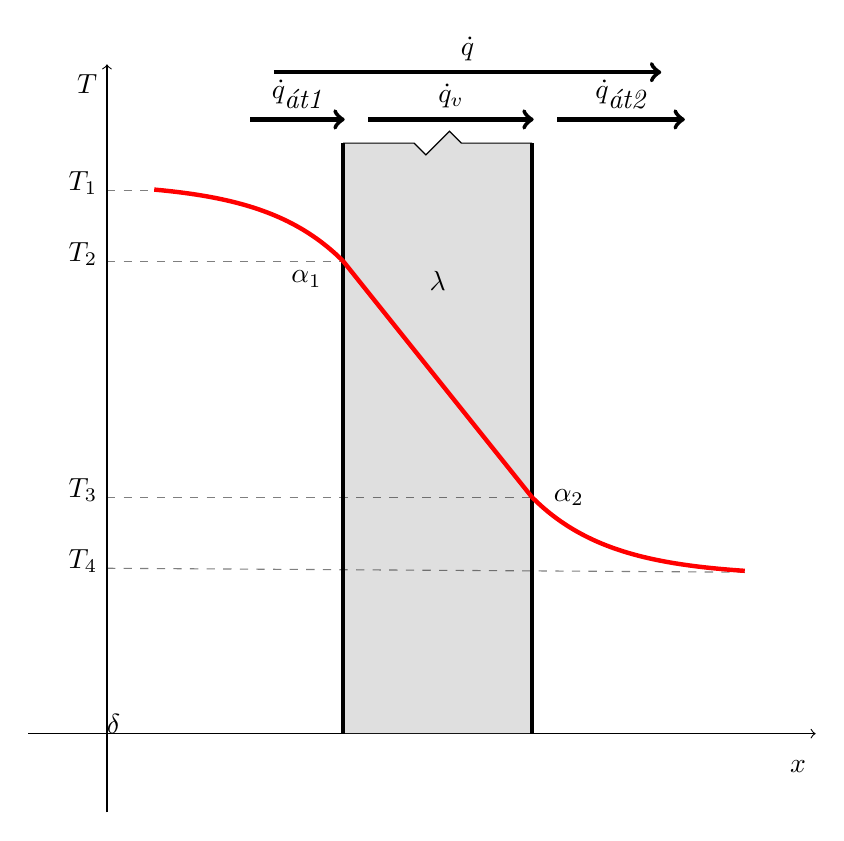
\begin{tikzpicture}
	
	\pgfmathsetmacro{\zoom}{1.5}
	\pgfmathsetmacro{\szel}{6*\zoom}
	\pgfmathsetmacro{\mag}{5*\zoom}
	\pgfmathsetmacro{\fal}{1.6*\zoom}
	\pgfmathsetmacro{\xdis}{2*\zoom}
	

	\pgfmathsetmacro{\Twegy}{4*\zoom}
	\pgfmathsetmacro{\Twketto}{2*\zoom}	

	\pgfmathsetmacro{\et}{\xdis+\fal}
	\pgfmathsetmacro{\von}{0.1*\zoom}
	% Tengelyek
	\draw[->] (0,-1) -- (0,\mag+1) node[anchor=north east]{$T$};
	\draw[->] (-1,0) -- (\szel,0) node[anchor=base east, shift={(0,-0.5)}]{$x$};
	
	%Fal
	\fill[gray,opacity=0.25](\xdis,0) -- (\xdis,\mag) --(\xdis+\fal/2-2*\von ,\mag) --(\xdis+\fal/2-\von ,\mag-\von) --(\xdis+\fal/2+\von ,\mag+\von)--(\xdis+\fal/2+2*\von ,\mag)-- (\et,\mag) -- (\et,0) -- (\xdis,0);
	
	\draw[ultra thick] (\xdis,0) -- (\xdis,\mag);
	
	\draw (\xdis,\mag)--(\xdis+\fal/2-2*\von ,\mag) --(\xdis+\fal/2-\von ,\mag-\von) --(\xdis+\fal/2+\von ,\mag+\von)--(\xdis+\fal/2+2*\von ,\mag)-- (\et,\mag) ;
	 
	\draw[ultra thick] (\et,\mag)-- (\et,0) ;
	
	%Szaggatott vonalak/felíratok
	\draw[black, opacity=0.5, dashed] (0,\Twegy+0.9) -- (\xdis*0.2,\Twegy+0.9);
	\node[anchor=base east] at (0,\Twegy+0.9) {$T_{1}$};		
	\draw[black, opacity=0.5, dashed] (0,\Twegy) -- (\xdis,\Twegy);
	\node[anchor=base east] at (0,\Twegy) {$T_{2}$};
	\draw[black, opacity=0.5, dashed] (0,\Twketto) -- (\xdis+\fal,\Twketto);
	\node[anchor=base east] at (0,\Twketto) {$T_{3}$};
	\draw[black, opacity=0.5, dashed] (0,\Twketto-0.9) -- (\et*1.5,\Twketto-0.95);
	\node[anchor=base east] at (0,\Twketto-0.9) {$T_{4}$};	

	%Hőmérséklet vonalak
	\draw[ultra thick, red](\xdis,\Twegy)--(\xdis+\fal,\Twketto);
	\node[anchor=north east] at (\xdis-\von,\Twegy) {$\alpha_1$};
	\node[anchor=west] at (\xdis+\fal+\von,\Twketto) {$\alpha_2$};
	\node[anchor=north] at (\xdis+\fal/2,\Twegy) {$\lambda$};
	\draw[ultra thick, color=red, domain=\xdis*0.2:\xdis, smooth, variable=\r] plot (\r, {\Twegy+1 - (exp(\r-\xdis))});
	\draw[ultra thick, color=red, domain=\et:\et*1.5, smooth, variable=\r] plot (\r, {\Twketto-1 + (exp(-\r+\et))});
	
	%Méretvonal
	\pgflength[xa=\xdis, ya=0, xb=\xdis+\fal, yb=0,ra={1}]{$\delta$};
	
	% Hőáram és hőáramsűrűség
	\draw[->, ultra thick] (\xdis*0.6-\von,\mag+2*\von ) -- (\xdis-\von,{\mag+2*\von}) node[midway, anchor=south]{$\dot{q}_{\textit{át1}}$} ;
	\draw[->, ultra thick] (\xdis+\von,\mag+2*\von ) -- (\et-\von,{\mag+2*\von}) node[midway, anchor=south]{$\dot{q}_v$} ;
	\draw[->, ultra thick] (\et+\von,\mag+2*\von ) -- (\et*1.3+\von,{\mag+2*\von}) node[midway, anchor=south]{$\dot{q}_{\textit{át2}}$} ;
	\draw[->, ultra thick] (\xdis*0.6+\von,\mag+6*\von ) -- (\et*1.3-\von,{\mag+6*\von}) node[midway, anchor=south]{$\dot{q}$} ;
	
	\end{tikzpicture}
	\caption{Hőmérséklet-hely függvény}
\end{figure}

\noindent A hőáramsűrűség a rendszerben létrejövő hőátadások és hővezetések esetén is megegyezik. 

\begin{equation}\label{e:mdpm86_elso}
\begin{split}
&\dot{q}=\dot{q}_{\textit{át1}} =\dot{q}_v=\dot{q}_{\textit{át2}}\\&\dot{q}=\alpha_1 (T_1-T_2)= \dfrac{\lambda_1}{\delta_1} (T_2 - T_3) = \alpha_2 (T_3-T_4)
\end{split}
\end{equation} 

\noindent A tagokat összevonva a következő összefüggést kapjuk.

\begin{equation}
T_1-T_4=\dot{q}\left(\dfrac{1}{\alpha_1}+\dfrac{\delta}{\lambda}+\dfrac{1}{\alpha_2}\right)
\end{equation} 

\noindent Ebből $\dot{q}$-t kifejezve az alábbi egyenletet kapjuk.

\begin{equation}
\dot{q}=\dfrac{T_1-T_4}{\dfrac{1}{\alpha_1}+\dfrac{\delta}{\lambda}+\dfrac{1}{\alpha_2}}
\end{equation} 

\noindent Ahol a hőátadási tényezőket és hővezetési tényezőt a következő módon vonhatjuk össze.

\begin{equation}
\kappa=\dfrac{1}{\dfrac{1}{\alpha_1}+\dfrac{\delta}{\lambda}+\dfrac{1}{\alpha_2}}=\dfrac{1}{\dfrac{1}{\SI{1162}{\watt\per\meter\squared\kelvin}}+\dfrac{\SI{0,016}{\meter}}{\SI{44,652}{\watt\per\meter\kelvin}}+\dfrac{1}{\SI{581,5}{\watt\per\meter\squared\kelvin}}}=\SI{340,38}{\watt\per\meter\squared\kelvin}
\end{equation} 

\noindent A hőáramsűrűség ezután a teljes hőmérséklet különbség és a $\kappa$ szorzataként számítható.

\begin{equation}
\dot{q}=\kappa(T_1-T_4)=\SI{340,38}{\watt\per\meter\squared\kelvin}(\SI{400}{\degreeCelsius}-\SI{200}{\degreeCelsius})=\SI{68076,71}{\watt\per\meter\squared}
\end{equation}

\noindent Ismerve a hőáramsűrűség értékét kiszámolhatjuk a hőfokeséseket. Az ehhez szükséges egyenletek kifejezhetőek az \ref{e:mdpm86_elso} egyenletből.

\begin{equation}
T_1-T_2=\dfrac{1}{\alpha_1}\dot{q}=\dfrac{1}{\SI{1162}{\watt\per\meter\squared\kelvin}}\SI{68076,71}{\watt\per\meter\squared}=\SI{58,54}{\kelvin}=\SI{58,54}{\degreeCelsius}
\end{equation}

\begin{equation}
T_3-T_4=\dfrac{1}{\alpha_2}\dot{q}=\dfrac{1}{\SI{581,5}{\watt\per\meter\squared\kelvin}}\SI{68076,71}{\watt\per\meter\squared}=\SI{117,07}{\kelvin}=\SI{117,07}{\degreeCelsius}
\end{equation}
